%%=============================================================================
%% Shortlist
%%=============================================================================

\chapter{\IfLanguageName{dutch}{Selectie van tools}{Selection of tools}}
\label{ch:shortlist}
Hierna volgen enkele beslissingen rond de gebruikte tools en technologie\"en in het technische luik van deze paper.
De vereisten van de opdrachtgever staan hierbij centraal zoals besproken in de~\nameref{sec:onderzoeksdoelstelling}.
Daarnaast komt ook een korte uitleg rond de keuze voor het te testen fitnessinstrument aan bod.
Het volgende hoofdstuk beschrijft vervolgens de uitwerking van dit luik met de gekozen tools in de vorm van een proof-of-concept.

\section{Android-app met Jetpack Compose}
\label{sec:keuze-framework-voor-android-app}
TODO Verder uitleggen (native, Jetpack Compose)

\section{Achterliggende service met Quarkus}
\label{sec:keuze-framework-voor-back-end}
TODO Verder uitleggen (Quarkus Dev Services en extensies, Langchain4j, Docker/Testcontainers, Kotlin in plaats van Java)

\section{Gemini als AI-platform}
\label{sec:keuze-ai-platform}
TODO Verder uitleggen (Google Gemini 1.5 Pro)

\section{Build tool}
\label{sec:build-tool}
Moderne software projecten maken tegenwoordig gebruik van een \textit{build tool}, wat helpt bij vele taken binnen het ontwikkelingsproces.
Bovendien is dit een vereiste voor complexere applicaties waar enkele tussenstappen vereist zijn, zoals bij het bouwen van een Android-applicatie.
Eveneens vergemakkelijkt het gebruik van een bouwsysteem om de proof-of-concept reproduceerbaar te houden.

\subsection{Voordelen van een build tool}
\label{subsec:voordelen-van-een-build-tool}
\textcite{Kandhway2019}~beschrijven de vijf grootste voordelen van het gebruiken van een build tool:
\begin{itemize}
    \item \textbf{Het automatiseert het bouwproces van software.}
    Software moet eerst gecompileerd worden om leesbaar en uitvoerbaar te zijn door een machine.
    Dit is automatiseerbaar aan de hand van een build tool, wat zal helpen bij het~\nameref{subsec:reproduceren-van-de-proof-of-concept}.
    \item \textbf{Het vergemakkelijkt het beheren van afhankelijkheden.}
    De achterliggende Quarkus service en de Android app zullen gebruik maken van libraries om het ontwikkelingsproces te vereenvoudigen.
    Een voorbeeld hiervan is het gebruik van de Quarkus REST-extensie, wat het verwerken van appgebruikers' verzoeken versoepelt.
    \item \textbf{Het verzekert het correct uitvoeren van het bouwproces.}
    Het bouwproces bestaat uit verschillende stappen die ondergaan moeten worden.
    Een build tool helpt hierbij om sommige stappen voor ons te bepalen, zoals de volgorde waarin afhankelijkheden inladen.
    \item \textbf{Het bespaart tijd door taken in parallel uit te voeren.}
    De build tool splitst taken op om gelijktijdig uit te voeren.
    Dit versnelt het bouwproces.
    \item \textbf{Het is een vereiste voor het toepassen van continuous integration.}
    \textit{Continuous integration} maakt het mogelijk om vooraf gedefinieerde bouwprocessen te lanceren eens er nieuwe code beschikbaar komt.
\end{itemize}

\subsection{Gradle}
\label{subsec:gradle}
Binnen het Java-ecosysteem staan Apache Maven en Gradle centraal als build tools.
Bij sommige oudere applicaties is het Ant-bouwsysteem nog in gebruik.
Het Kotlin-ecosysteem kent de voorkeur naar Maven en Gradle gezien haar oorspronkelijk ontwerp om interoperabiliteit met Java te verzekeren.
Google, de ontwikkelaars achter het Jetpack Compose framework en het Android besturingssysteem, hebben ervoor gekozen om uitsluitend met Gradle te werken wegens de beperktheid van Maven op vlak van bouwprocessen opstellen.
Met de keuze voor Jetpack Compose zoals besproken in~\ref{sec:keuze-framework-voor-android-app} zal daarmee ook gebruik gemaakt worden van Gradle voor de achterliggende Quarkus service.
De reden hiervoor is om het bouwproces zo gestroomlijnd en consistent mogelijk te houden tussen de te ontwikkelende platformen, de visualisatie van dit bouwproces is te zien in~\ref{fig:visualisatie-gradle-bouwproces}.
Een bijkomend voordeel is de mogelijkheid om de Kotlin-syntax te gebruiken binnen Gradlebestanden.
\begin{figure}
    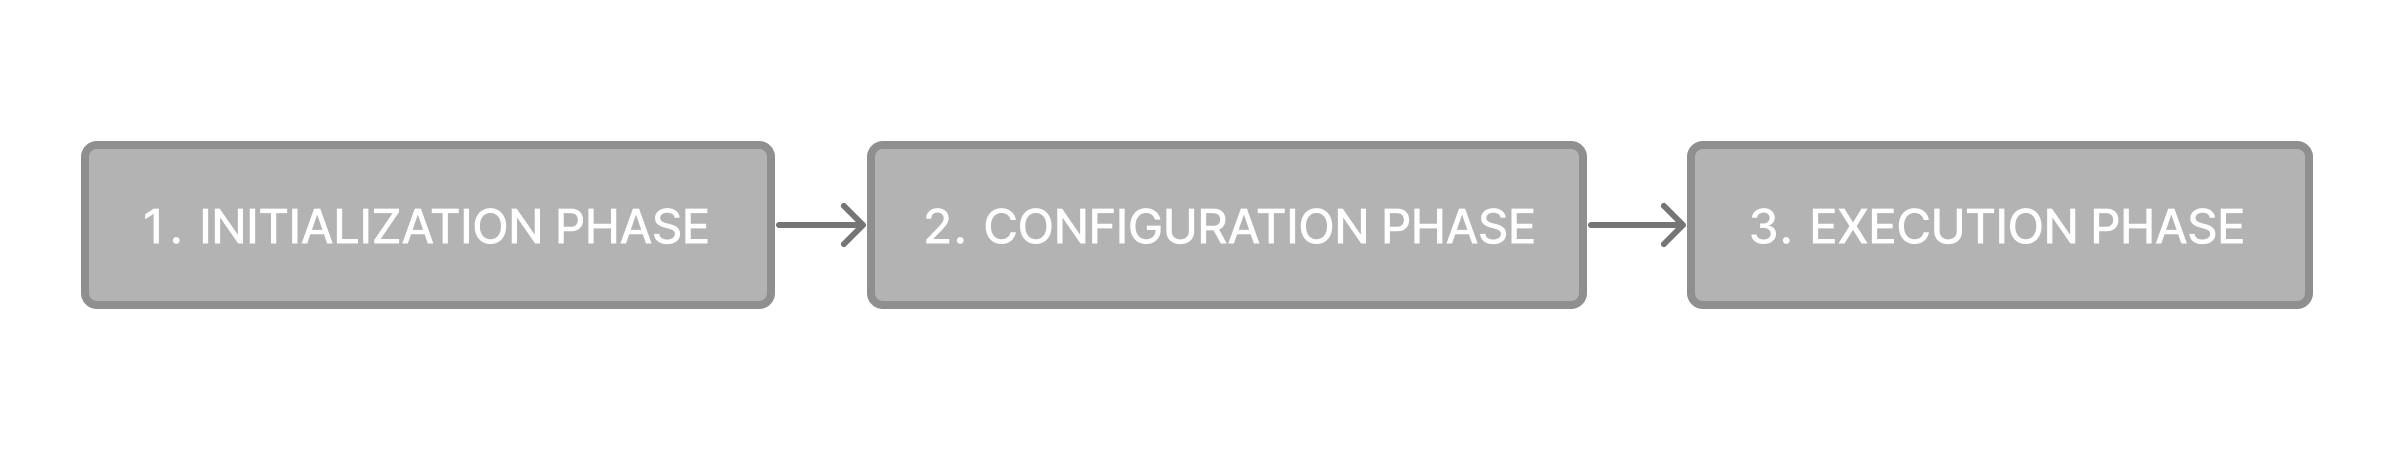
\includegraphics[width=1\linewidth]{images/gradle-buildprocess}
    \caption{De drie stappen in het Gradle bouwproces~\autocite{Gradle}}
    \label{fig:visualisatie-gradle-bouwproces}
\end{figure}

\section{Gekozen fitnessinstrument}
\label{sec:gekozen-fitnessinstrument}
TODO